\section{Endliche Akzeptoren}
\begin{frame}{Endliche Akzeptoren}
	\begin{Definition}
		Ein endlicher Akzeptor ist ein Moore-Automat mit $ Y= \{0,1\}$, der $1$ ausgibt, falls das eingegebene Wort der vorliegenden Syntax entspricht und $0$ sonst.
	\end{Definition} 

	\emph{Notation} : Wir kennzeichnen akzeptierende Zustände mit einem Doppelkreis. \\ \pause
	
	Wir sprechen von einer akzeptierten Sprache über einem Alphabet. Sie ist definiert als $$ L = \{ w \mid g_*(z_0,w) = 1 \} $$ 
	Also sind in einer akzeptierten Sprache alle Wörter, die akzeptiert werden.
\end{frame}

% TODO
\begin{frame}{}
\end{frame}

%% Übung: Beispiel
\setbeamercolor{background canvas}{bg=}
\includepdf[pages=44]{U12.pdf}

\begin{frame}{Aufgabe}
	Der endliche Akzeptor $A = (Z, z_0, X, f, F)$ sei gegeben durch
	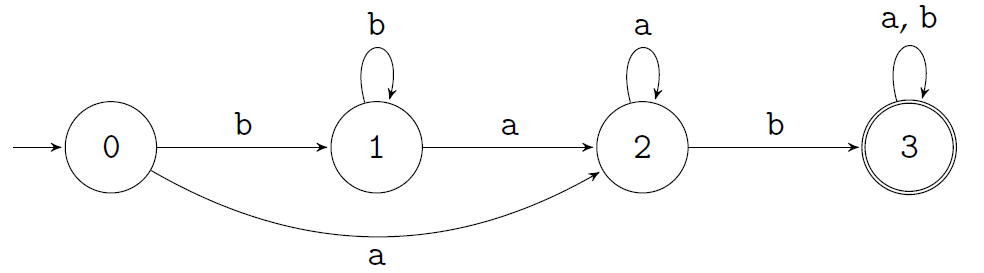
\includegraphics[scale=0.4]{automaten/akz1516B12A1}
	
	Geben Sie die von $A$ akzeptierte Sprache $L(A)$, unter ausschließlicher Benutzung der formalen Sprachen $\{\#a\}$, $\{\#b\}$, sowie $\{\#a, \#b\}$, des Konkatenationsabschlusses und des Produkts formaler Sprachen, an.
	
	\emph{Beispiel:} $\{\#a, \#b\}^* \cdot \{\#a\} \cdot \{\#b\}$
	
	\only<2-|handout:2>{
		\begin{block}{Lösung}
			$L(A) = \{\#b\}^* \cdot \{\#a\} \cdot \{\#a\}^* \cdot \{\#b\} \cdot \{\#a, \#b\}^*$
		\end{block}
	}
\end{frame}

\begin{frame}{Aufgabe}
	\begin{itemize}
		\item Zeichnen Sie einen möglichst kleinen endlichen Akzeptor mit $ X = \{a,b\}$, der alle Wörter akzeptiert, bei denen die Anzahl der $a$ durch $5$ teilbar ist.
		\item Zeichnen Sie einen Akzeptor mit $ X = \{a,b\}$, der alle Wörter akzeptiert, in denen nirgends hintereinander zwei $b$ vorkommen.
	\end{itemize}		
\end{frame}
\begin{frame} 
	\frametitle{Lösung}
	\only<1|handout:1>{ \begin{figure}[H] 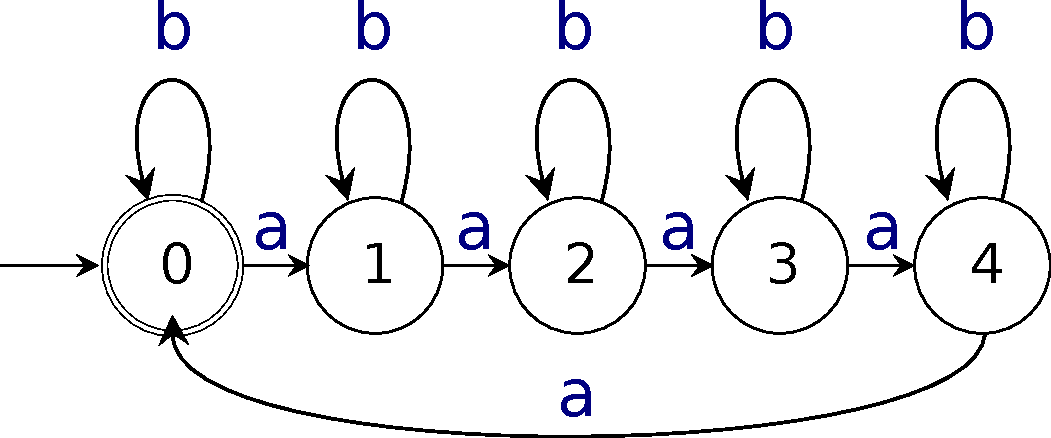
\includegraphics[scale=0.5]{automaten/Akzeptor1.pdf} \end{figure}}		
	\only<2|handout:2>{ \begin{figure}[H] 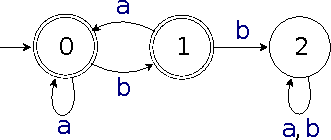
\includegraphics[scale=1.5]{automaten/Akzeptor2.pdf} \end{figure}}
\end{frame} 

